%=================AVANCES Y PRUEBAS=================
% SENSORES DE PULSO

\section{Módulo Gestion de Vehiculos}
Dentro de los modulos importantes que contribuyen al buen funcionamiento de "In-Help" encontramos el modulo Gestion de vehiculos dentro de el podremos obtener la información correspondiente a placas del automovil como tambien numero y fecha de vencimiento de polizas de seguro . Dentro de el encontraremos el siguiente flujo.\\



\subsection{Registrar Vehiculos}

La figura \ref{fig:RegistraVehiculo} se muestra el diagrama de secuencia correspondiente al envío de registro de un nuevo vehiculo, donde se utiliza la comunicación con la base de datos para la creación de un nuevo vehiculo.

\begin{figure}[htbp!]
	\centering
	\fbox{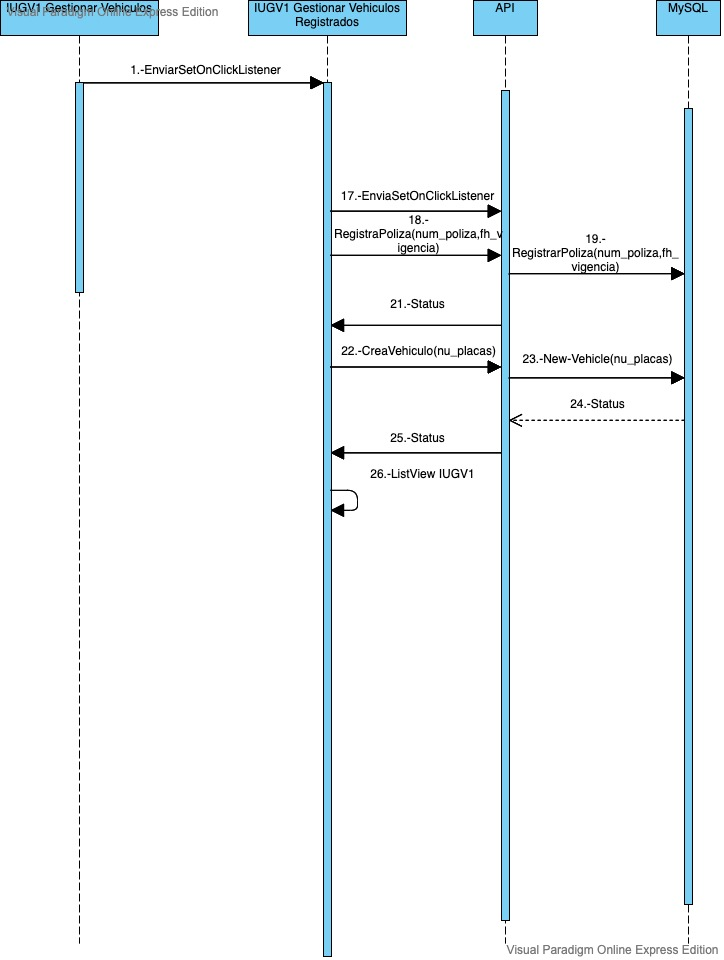
\includegraphics[width=1.0\textwidth]{AvancesPruebas/imagenes/Registra_Vehiculo}}
	\caption{Diagrama secuencia del registo de vehiculos}
	\label{fig:RegistraVehiculo}
\end{figure}
\begin{itemize}
	\item \textbf{Envia.setOnClickListener:} La información que sera enviada en caso de querer registrar un nuevo vehiculo para un usuario.
	\item \textbf{CreaVehiculo(nu_placas):} Realiza la peticion a el API para poder ingresar un numero de placas nuevo.
	\item \textbf{New-Vehicle(nu_placas):} Es el metodo POST que realiza la insercion de el numero de placas a la Base de datos.
	\item \textbf{Status):} Regresa el status correspondiente a el query realizado dentro de la base de datos.
	\item \textbf{RegistraPoliza(num_poliza,fh_vigencia):} Es el metodo POST correspondiente a la inserción de una poliza de seguro acorde a su numero y fecha de vigencia.
	\item \textbf{ListView IUGV1:} Carga la lista de automoviles registrados para ese usuario.

\end{itemize}

\subsection{Obtener Vehiculos Registrados}

La figura \ref{fig:ObtencionVehiculos} se muestra el diagrama de secuencia correspondiente a la obtencion de los vehiculos registrados para correspondientes a ese usuario. Donde se utiliza la comunicación con la base de datos para la obtención de todos los vehiculos.

\begin{figure}[htbp!]
	\centering
	\fbox{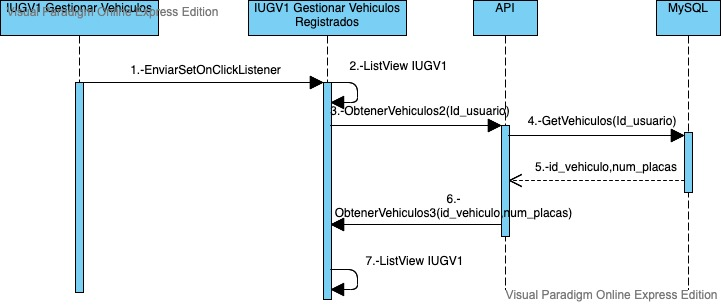
\includegraphics[width=1.0\textwidth]{AvancesPruebas/imagenes/IUGV1_1}}
	\caption{Diagrama secuencia de Obtencion de vehiculos registrados}
	\label{fig:ObtencionVehiculos}
\end{figure}
\begin{itemize}
	\item \textbf{Envia.setOnClickListener:} La información que sera enviada en caso de querer registrar un nuevo vehiculo para un usuario.
	\item \textbf{ObtenerVehiculos2(id_usuario)):} Realiza una peticion a el API para la obtencion de los vehiculos registrados.
	\item \textbf{GetVehiculos(id_usuario):} Realiza la peticion GET correspondiente a una busqueda dentro de la base de datos acorde a dicho usuario.
	\item \textbf{id_vehiculo,num_placas:} Regresa a el API los datos correspondientes mencionados anteriormente.
	\item \textbf{ObtenerVehiculos3(id_vehiculo,num_placas):} Obtiene los datos correspondientes a la petición realizada al SGBD.
	\item \textbf{ListView IUGV1:} Carga la lista de automoviles registrados para ese usuario.

\end{itemize}

La figura \ref{fig:ActualizarVehiculos} se muestra el diagrama de secuencia correspondiente a la actualizacion de datos correspodiente  a un vehiculo registrado. Se realiza interaccion con el API y base de datos para la actualizacion de dicha informacion

\begin{figure}[htbp!]
	\centering
	\fbox{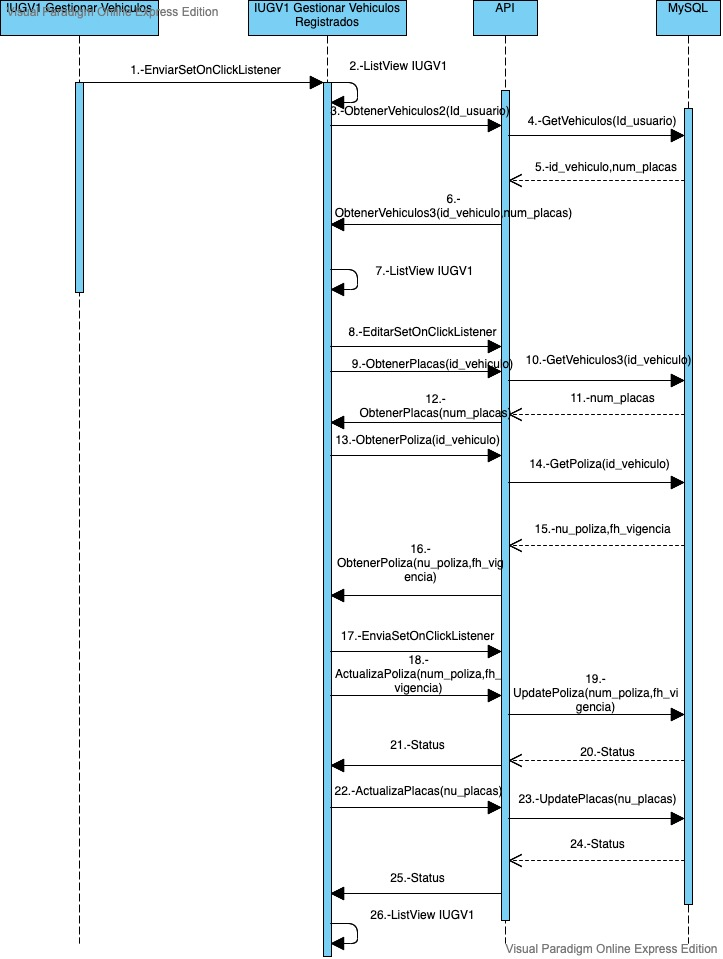
\includegraphics[width=1.0\textwidth]{AvancesPruebas/imagenes/IUGV1_1_1.vpd}}
	\caption{Diagrama secuencia de Obtencion de vehiculos registrados}
	\label{fig:ActualizarVehiculos}
\end{figure}
\begin{itemize}
	\item \textbf{Envia.setOnClickListener:} La información que sera enviada en caso de querer registrar un nuevo vehiculo para un usuario.
	\item \textbf{ObtenerVehiculos2(id_usuario)):} Realiza una peticion a el API para la obtencion de los vehiculos registrados.
	\item \textbf{GetVehiculos(id_usuario):} Realiza la peticion GET correspondiente a una busqueda dentro de la base de datos acorde a dicho usuario.
	\item \textbf{id_vehiculo,num_placas:} Regresa a el API los datos correspondientes mencionados anteriormente.
	\item \textbf{ObtenerVehiculos3(id_vehiculo,num_placas):} Obtiene los datos correspondientes a la petición realizada al SGBD.
	\item \textbf{ListView IUGV1:} Carga la lista de automoviles registrados para ese usuario.
	\item \textbf{Editar.setOnClickListener:} Realiza la peticion UPDATE correspondiente a una actualizacion de datos dentro del SGBD.
	\item \textbf{ObtenerPlacas(id_vehiculo):} Peticion al API para la obtencion del dato seleccionado en dicha pantallas.
	\item \textbf{GetVehiculos3(id_vehiculo):} Petiion tipo GET para muestreo dentro de la Base de datos correspondiente a los atributos anteriormente mencionados.
	\item \textbf{num_placas:} Datos pedidos por la peticion anterior.
	\item \textbf{ObtenerPoliza(id_vehiculo):} Peticion al API para la obtencion del dato seleccionado en dicha pantallas.
	\item \textbf{GetPoliza(id_vehiculo):} Petiion tipo GET para muestreo dentro de la Base de datos correspondiente a los atributos anteriormente mencionados.
	\item \textbf{num_poliza,fh_vigencia:} Datos pedidos por la peticion anterior.
	\item \textbf{ActualizaPoliza(num_poliza,fh_vigencia):} Peticion API para la actualizacion de datos.
	\item \textbf{UpdatePoliza(num_poliza,fh_vigencia):} Actualizacion de tipo UPDATE dentro de la base de datos con los parametros anteriormente mencionados.
	\item \textbf{ActualizaPlacas(num_placas):} Peticion API para la actualizacion de datos.
	\item \textbf{UpdatePlacas(num_placas):} Actualizacion de tipo UPDATE dentro de la base de datos con los parametros anteriormente mencionados.
	\item \textbf{Status):} Regresa el status correspondiente a el query realizado dentro de la base de datos.



\end{itemize}



